\documentclass[11pt,a4paper]{article}
\usepackage[utf8]{inputenc}
\usepackage[T1]{fontenc}

\usepackage[margin=2cm]{geometry}
\usepackage[x11names]{xcolor}
\usepackage{array,multirow,graphicx}
\usepackage{amsmath,amssymb}
\usepackage{enumitem}
\setlist{itemsep=1pt,topsep=1pt,parsep=1pt,partopsep=1pt}
\usepackage{tikz}
\usetikzlibrary{shapes.geometric}
\usepackage{cleveref}
\usepackage{listings}
\lstset{
	basicstyle=\ttfamily\small,
	keywordstyle=\color{Firebrick4},
	commentstyle=\color{RoyalBlue4},
	identifierstyle=\color{black},
	stringstyle=\color{SpringGreen4},
}

\newcommand{\MadNkLO}[0]{\sc{MadNkLO}}

\title{Generation of counterterms in \MadNkLO}
\author{Simone Lionetti}
\date{\today}


\begin{document}

\maketitle

This document describes the contents of the file \texttt{subtraction.py}
(located in \texttt{madgraph/core}).


\section{Classes}


\subsection{\texttt{SubtractionLeg}}
\label{ssec:subtractionleg}

For the purpose of the subtraction,
it is impractical to carry around the whole information
that is contained in an object of the type \texttt{base\_objects.Leg}.
A simpler object \texttt{SubtractionLeg} is therefore defined
with the following three attributes:
\begin{itemize}
	\item \texttt{n}: an integer that indicates the leg number in the process,
	\item \texttt{pdg}: the PDG identifier which specifies the type of particle,
	\item \texttt{state}: a flag to specify if the leg
		is in the initial or in the final state.
\end{itemize}

For convenience, a class \texttt{SubtractionLegSet} which represents
a set of \texttt{SubtractionLeg}s is also implemented.
Internally, this is just a sorted \texttt{tuple} since it is assumed
that order is irrelevant.
However, this object also provides some additional useful methods.


\subsection{\texttt{SingularStructure}}
\label{ssec:singularstructure}

The \texttt{SingularStructure} class is designed to identify
unresolved regions of phase space, and by extension counterterms.
It is a recursive structure which represents a tree of \texttt{SubtractionLeg}s
in a process.
At each level, the leaves are gathered
into a \texttt{SubtractionLegSet} attribute called `\texttt{legs}'
and the \texttt{SingularStructure} that specify sub-trees are grouped
into a \texttt{list} called `\texttt{substructures}'.
There are currently three classes that inherit from \texttt{SingularStructure}
and represent different types of phase space regions:
\begin{itemize}
	\item \texttt{SoftStructure} indicates that all of its sub-legs are soft,
	\item \texttt{CollStructure} indicates
		that all of its sub-legs are collinear,
	\item \texttt{BeamStructure} specifies that a leg is taken from a hadron
		beam after some splitting.
\end{itemize}
The generic parent class \texttt{SingularStructure} can be instantiated
to group together several structures and specify an additional set of legs;
this feature is exploited in the implementation of momentum mappings
to specify recoilers.

For the sake of concreteness,
a non-trivial example of \texttt{SingularStructure}
is illustrated in \cref{fig:singularstructure}.
In the conversion to a string, by default the PDGs and the state labels
of \texttt{SubtractionLeg}s are suppressed,
and \texttt{SingularStructure}s are converted to a single character
such that the object of \cref{fig:singularstructure} prints as
\begin{equation}
	\texttt{C(C(C(5,13),C(7,10,11,16)),S(4,6,8),1,9)}.
\end{equation}
The conversion of objects to characters is carried out
through the method \texttt{name}, according to the rules
\begin{equation}
\begin{aligned}
	&\texttt{SingularStructure} \to \texttt{`'}, &
	&\texttt{CollStructure} \to \texttt{`C'}, \\
	&\texttt{SoftStructure} \to \texttt{`S'}, &
	&\texttt{BeamStructure} \to \texttt{`F'}.
\end{aligned}
\end{equation}

\begin{figure}
\centering
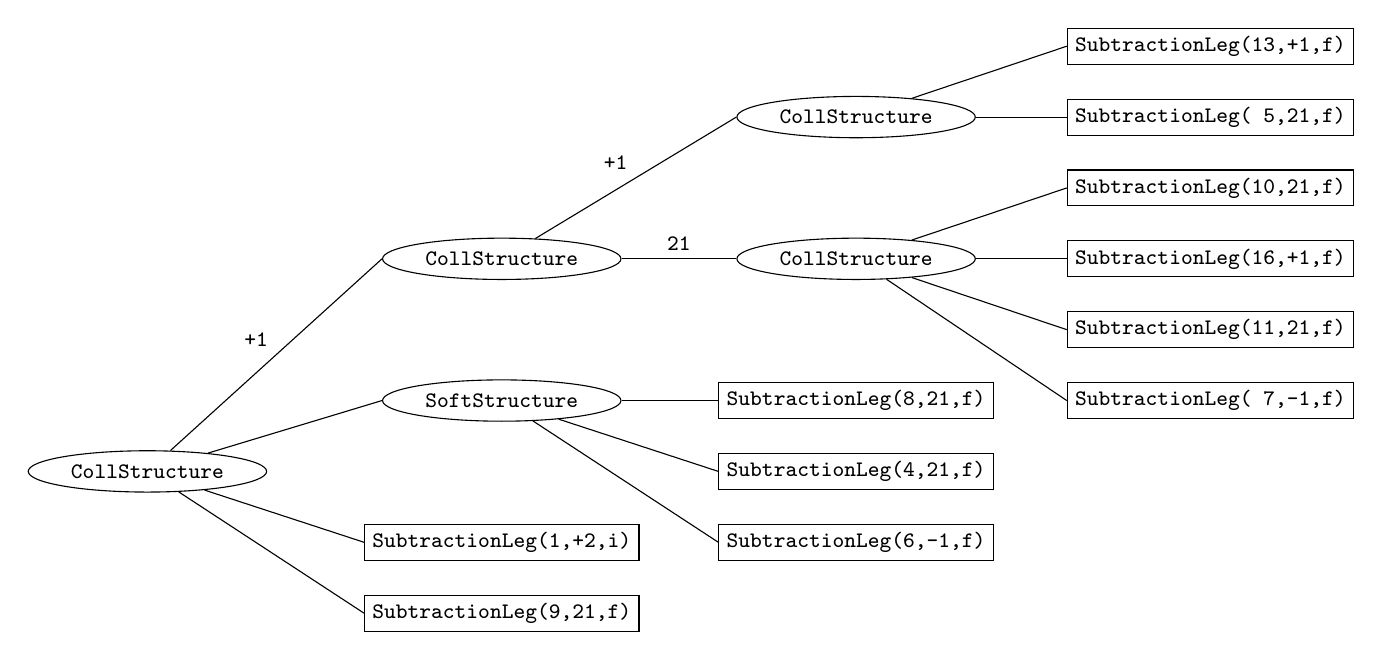
\begin{tikzpicture}[scale=0.9]
\footnotesize
	\draw (0,  0) node[ellipse,draw] (C1)  {\tt{CollStructure}};
	\draw (5, +3) node[ellipse,draw] (C2)  {\tt{CollStructure}};
	\draw (5, +1) node[ellipse,draw] (S2)  {\tt{SoftStructure}};
	\draw (10,+3) node[ellipse,draw] (C3a) {\tt{CollStructure}};
	\draw (10,+5) node[ellipse,draw] (C3b) {\tt{CollStructure}};
	\draw (5, -1) node[draw] (leg2a) {\tt{SubtractionLeg(1,+2,i)}};
	\draw (5, -2) node[draw] (leg2b) {\tt{SubtractionLeg(9,21,f)}};
	\draw (10,-1) node[draw] (leg3a) {\tt{SubtractionLeg(6,-1,f)}};
	\draw (10, 0) node[draw] (leg3b) {\tt{SubtractionLeg(4,21,f)}};
	\draw (10,+1) node[draw] (leg3c) {\tt{SubtractionLeg(8,21,f)}};
	\draw (15,+1) node[draw] (leg4a) {\tt{SubtractionLeg( 7,-1,f)}};
	\draw (15,+2) node[draw] (leg4b) {\tt{SubtractionLeg(11,21,f)}};
	\draw (15,+3) node[draw] (leg4c) {\tt{SubtractionLeg(16,+1,f)}};
	\draw (15,+4) node[draw] (leg4d) {\tt{SubtractionLeg(10,21,f)}};
	\draw (15,+5) node[draw] (leg4e) {\tt{SubtractionLeg( 5,21,f)}};
	\draw (15,+6) node[draw] (leg4f) {\tt{SubtractionLeg(13,+1,f)}};
	\draw (C1) edge node[above left] {\tt{+1}} (C2.west);
	\draw (C1) edge (S2.west);
	\draw (C1) edge (leg2a.west);
	\draw (C1) edge (leg2b.west);
	\draw (S2) edge (leg3a.west);
	\draw (S2) edge (leg3b.west);
	\draw (S2) edge (leg3c.west);
	\draw (C2) edge node[above] {\tt{21}} (C3a.west);
	\draw (C2) edge node[above left] {\tt{+1}} (C3b.west);
	\draw (C3a) edge (leg4a.west);
	\draw (C3a) edge (leg4b.west);
	\draw (C3a) edge (leg4c.west);
	\draw (C3a) edge (leg4d.west);
	\draw (C3b) edge (leg4e.west);
	\draw (C3b) edge (leg4f.west);
\end{tikzpicture}
\caption{
Example scheme of a \texttt{SingularStructure} object.
The nodes in bubbles belong to the list of \texttt{substructure}
of the structure they are linked to on the left,
while the ones in boxes belong to its \texttt{legs}.
Within \texttt{SubtractionLeg} objects, initial and final states
are here abbreviated with the letters \texttt{i} and \texttt{f} respectively.
}
\label{fig:singularstructure}
\end{figure}


\section{Generation of elementary operators}
\label{sec:operators}

Given a process, the first 

\begin{thebibliography}{9}

\end{thebibliography}

\end{document}
